\documentclass[tikz,border=10pt]{standalone}
\usetikzlibrary{positioning, shapes, arrows.meta}
\begin{document}
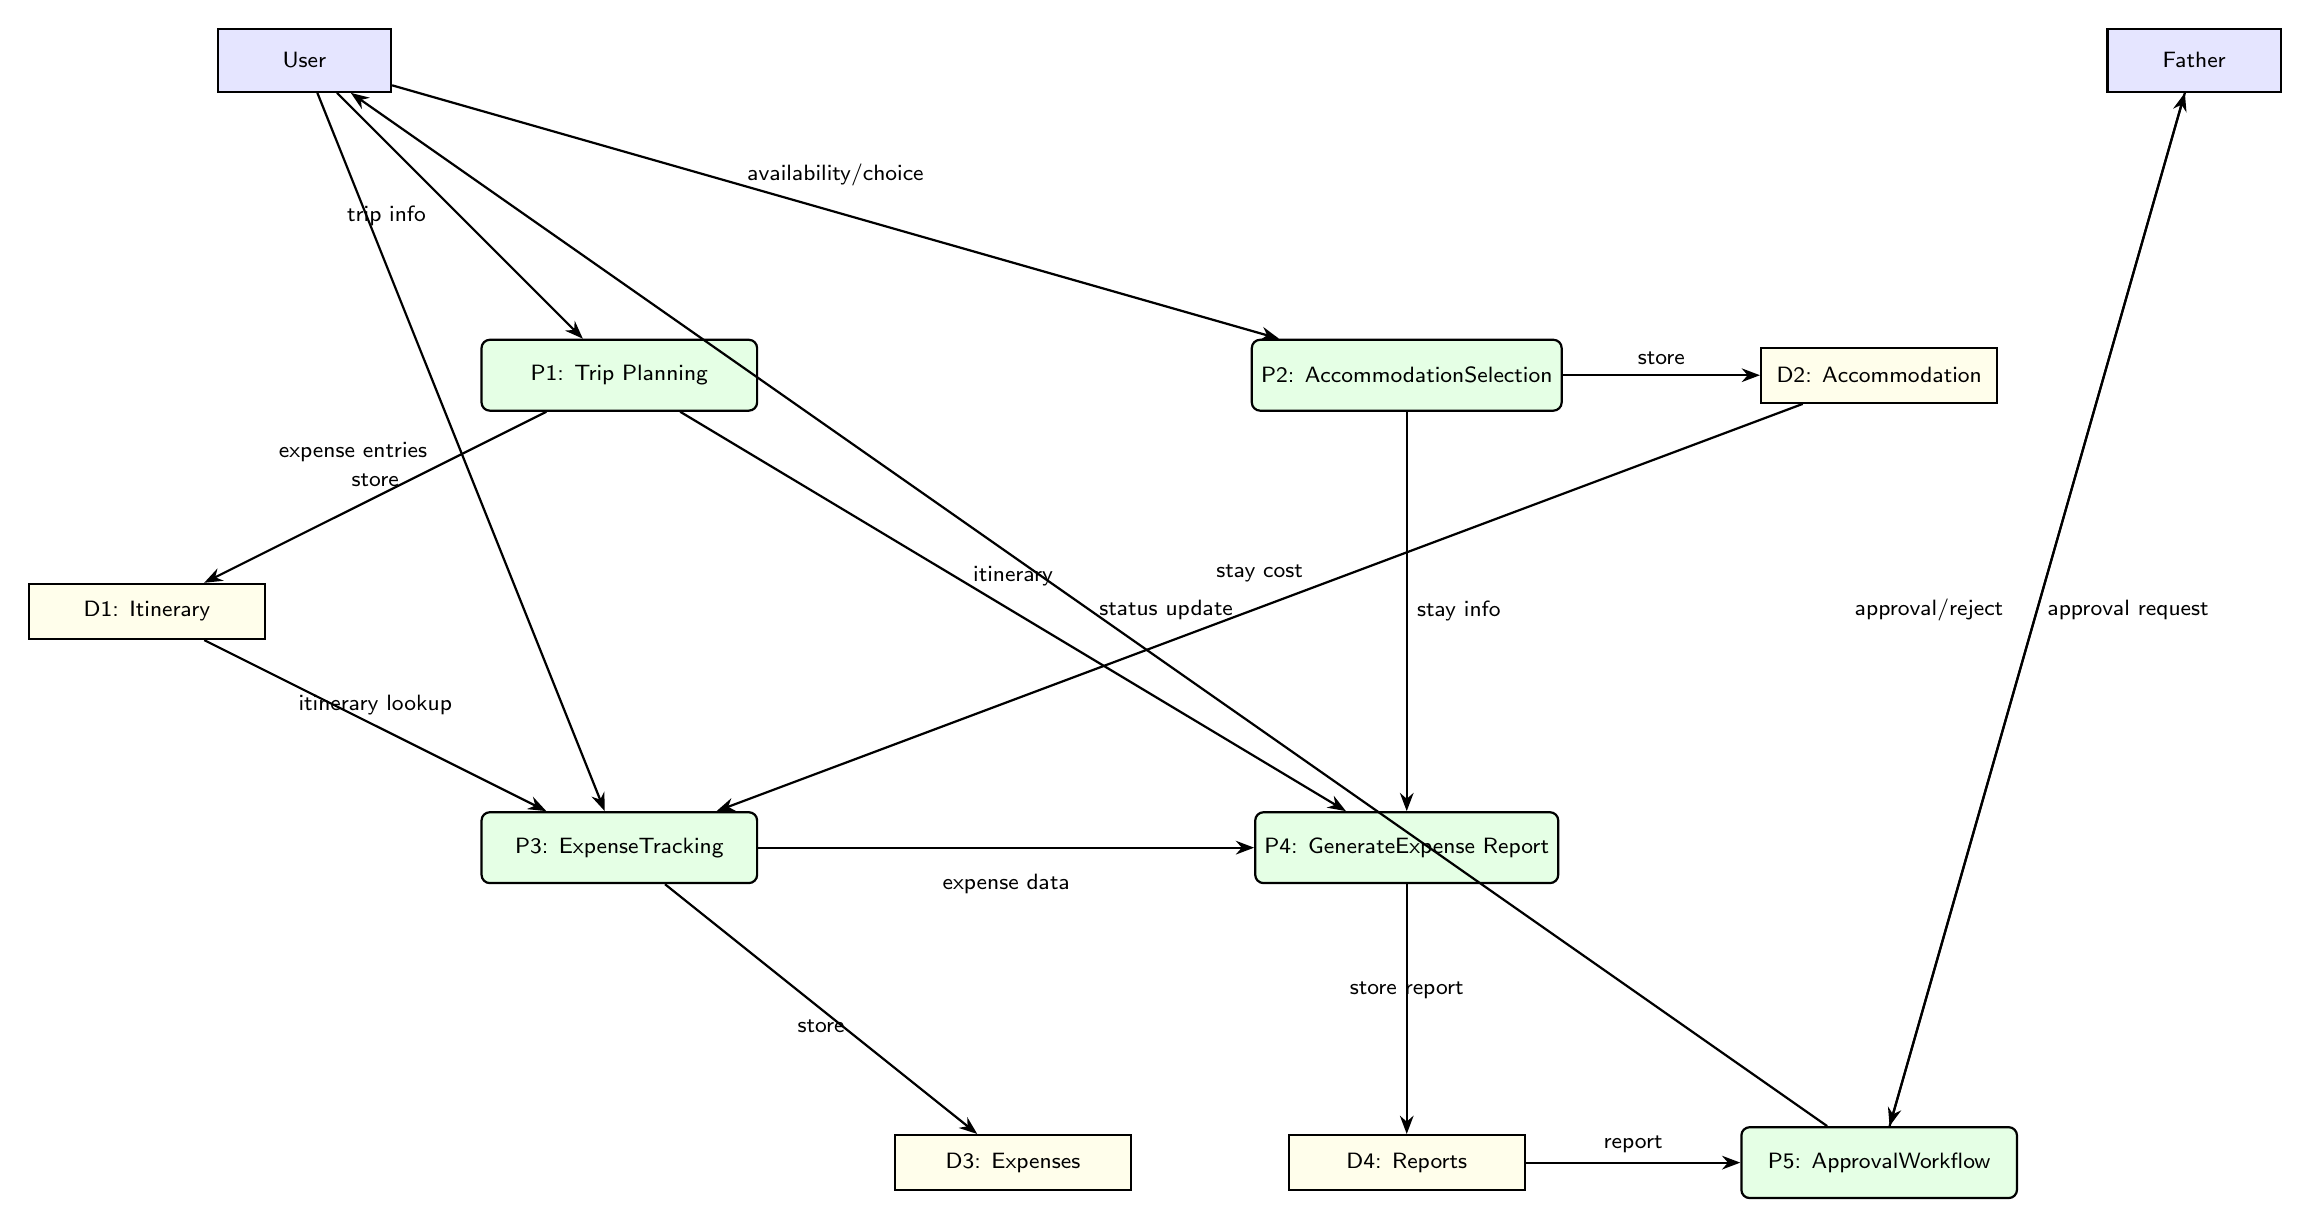
\begin{tikzpicture}[every node/.style={font=\sffamily\footnotesize}]
  % Styles
  \tikzset{
    external/.style={rectangle, draw=black, thick, minimum width=22mm, minimum height=8mm, fill=blue!10},
    process/.style={rectangle, rounded corners=3pt, draw=black, thick, minimum width=35mm, minimum height=9mm, fill=green!10},
    datastore/.style={draw, thick, minimum width=30mm, minimum height=7mm, fill=yellow!8},
    flow/.style={->, >=Stealth, thick}
  }
  
  % External entities - 2x more spacing
  \node[external] (user) at (0,16) {User};
  \node[external] (father) at (24,16) {Father};
  
  % Processes - 2x more spread out
  \node[process] (p1) at (4,12) {P1: Trip Planning};
  \node[process] (p2) at (14,12) {P2: Accommodation\\Selection};
  \node[process] (p3) at (4,6) {P3: Expense\\Tracking};
  \node[process] (p4) at (14,6) {P4: Generate\\Expense Report};
  \node[process] (p5) at (20,2) {P5: Approval\\Workflow};
  
  % Data stores - 2x more strategically positioned
  \node[datastore] (d1) at (-2,9) {D1: Itinerary};
  \node[datastore] (d2) at (20,12) {D2: Accommodation};
  \node[datastore] (d3) at (9,2) {D3: Expenses};
  \node[datastore] (d4) at (14,2) {D4: Reports};
  
  % Primary flows from User - straight lines
  \draw[flow] (user) -- (p1) node[midway, left, xshift=-3mm] {trip info};
  \draw[flow] (user) -- (p2) node[midway, above, yshift=2mm] {availability/choice};
  \draw[flow] (user) -- (p3) node[midway, left, xshift=-3mm] {expense entries};
  
  % Process to datastore flows - straight lines
  \draw[flow] (p1) -- (d1) node[midway, above] {store};
  \draw[flow] (p2) -- (d2) node[midway, above] {store};
  \draw[flow] (p3) -- (d3) node[midway, below] {store};
  \draw[flow] (p4) -- (d4) node[midway, above] {store report};
  
  % Inter-process flows - straight lines
  \draw[flow] (p1) -- (p4) node[midway, above, yshift=2mm] {itinerary};
  \draw[flow] (p2) -- (p4) node[midway, right] {stay info};
  \draw[flow] (p3) -- (p4) node[midway, below, yshift=-2mm] {expense data};
  
  % Approval workflow - straight lines
  \draw[flow] (d4) -- (p5) node[midway, above] {report};
  \draw[flow] (p5) -- (father) node[midway, right] {approval request};
  \draw[flow] (father) -- (p5) node[midway, left, xshift=-3mm] {approval/reject};
  \draw[flow] (p5) -- (user) node[midway, right] {status update};
  
  % Lookup flows - straight lines
  \draw[flow] (d1) -- (p3) node[midway, above] {itinerary lookup};
  \draw[flow] (d2) -- (p3) node[midway, above, yshift=2mm] {stay cost};
  
\end{tikzpicture}
\end{document}